\documentclass[12pt,fleqn]{article}
\setlength{\parindent}{0pt}
\usepackage{graphicx}
\usepackage{cancel}
\usepackage{listings}
\usepackage[latin5]{inputenc}
\usepackage{color}
\setlength{\parskip}{8pt}
\setlength{\parsep}{0pt}
\setlength{\headsep}{0pt}
\setlength{\topskip}{0pt}
\setlength{\topmargin}{0pt}
\setlength{\topsep}{0pt}
\setlength{\partopsep}{0pt}
\setlength{\mathindent}{0cm}

\begin{document}
Ders 17

Onceki derste 

\[ \int \int (1-x^2-y^2) dA \]

\[ x^2+y^2 \le 1 \]

\[ x,y \ge 0 \]

entegralini hesapladik, fakat kullandigimiz yontem biraz karmasikliga yol
acti. Daha iyi bir yontem kutupsal forma gecmektir. 

Hatirlarsak $x,y$ kordinat sisteminde cift entegral icin entegrasyon
alanini yatay, dikey sekilde parcalara ayirmistik, $dA = dy \ dx$ haline
gelmisti. Kutupsal formda 

\[ \int \int  ... \ dr \ d\theta\]

seklinde bir form olur, once $r$ uzerinden entegrasyon en kolayi. Bu
demektir ki $\theta$'yi sabitleriz, ve $r$ uzerinde hareket ederiz. 

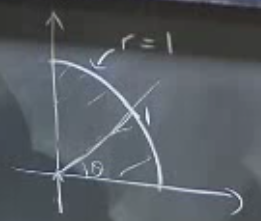
\includegraphics[height=3cm]{17_1.png}

Birim disk orneginde bu hareket basit, $r=0$'dan baslanir, ve 1 degerine
gelinceye kadar hareket edilir. $\theta$ icin 0'dan baslanir, ustteki alana
gore, $\pi/2$'ya gelinceye kadar hareket edilir. Sinirlar soyle olur:

\[ \int_0^{\pi/2} \int_0^1  ... \ dr \ d\theta\]

Fakat, dikkat, bu onemli bir nokta, $dA$ buyuklugu $dr \ d\theta$'ya esit
{\em degildir}. 

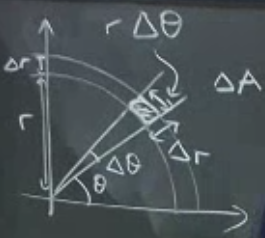
\includegraphics[height=3cm]{17_2.png}

Ustteki resimdeki ici karalanmis ufak dikdortgeni dusunelim, dikdortgenin
kenarlarindan biri biraz egimlidir (cemberin parcasi oldugu icin) fakat
kenarlar kuculdukce bu ufak alan dikdortgen olarak gorulebilir. Neyse,
kenarlarin biri $\Delta r$ (bu kolay), digeri? Oteki kenar $\Delta \theta$
degil, cunku o kenar cemberin bir parcasi, o zaman $r \ \Delta \theta$.

Bu demektir ki kenarlari sonsuz kuculttugumuz zamanda bile 

\[ dA = r \ dr \ d\theta \]

olacak. Entegral

\[ \int_0^{\pi/2} \int_0^1  f \ dr \ d\theta\]

\[ f =  (1-x^2-y^2)\]

Kutupsal forma tabii ki mekanik bir sekilde

\[ x = rcos\theta \]

\[ y = rsin\theta \]

esitliklerini alip $f$ icinde yerlerine koyabiliriz, fakat biraz dikkatli
bakarsak $-x^2-y^2$ aslinda $-(x^2+y^2)$ ve $r^2=x^2+y^2$ olduguna gore,
bunu kullanabiliriz

\[ f =   1-r^2 \]

Yani

\[ \int_0^{\pi/2} \int_0^1  1-r^2 \ dr \ d\theta\]


\[ \int_0^{\pi/2}  \bigg[ \frac{r^2}{2} - \frac{r^4}{4} \bigg]_0^1 \ d\theta\]


\[ \int_0^{\pi/2}  \frac{1}{4} \ d\theta = \frac{1}{4} \frac{\pi}{2} =
\frac{\pi}{8}
\]

Onceki derse gore daha kolay oldu. 

Cift entegraller ne ise yarar? 

Onceki derste cift entegralleri hacim hesaplama baglaminda isledik. Fakat
hacim hesabi tek uygulama alanlari degil, aynen tek degiskenli entegralin
sadece alan hesaplamada kullanilmadigi gibi. Cift entegralleri
belli bir bolgedeki fonksiyonlari toplama olarak gormek daha iyi [1], belki bu
fonksiyonun o bolgedeki ortalamasini hesaplamak istiyoruz, vs. Bazi
kullanimlari listeleyelim:

Uygulamalar 

1) Belli bir bolge $R$'nin alanini hesaplamak. 

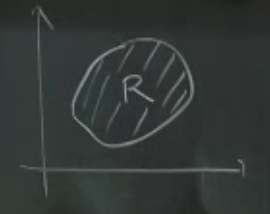
\includegraphics[height=2cm]{17_3.png}

Bazi durumlarda bu hesap tek entegral ile yapilabiliyor, ama cift entegral
ile daha kolay. Soyle

\[ Alan(R) = \int \int_R 1 \ dA \]

Eger cift entegralleri illa hacim olarak gormek istiyorsak, ustteki hesap
yuksekligi 1, baz alani $R$ olan bir ``hacmi'' hesapliyor. Hacim = baz alan
X yukseklik'tir, ama yukseklik 1 oldugu icin, ustteki hesap ayni sadece baz
alanin ne oldugunu hesaplar! Guzel bir cinlik degil mi?

Ya da, diyelim ki yassi / duz bir objenin kutlesini hesaplamak istiyoruz,
ve yogunluk $\delta = kutle / \textit{birim alan}$ olarak verilmis. Her
ufak parca icin kutle

\[ \Delta m = \delta \cdot \Delta A \]

Tum kutleyi ustteki ufak kutleleri toplayarak elde edebiliriz. 

\[ \int \int_R \delta \cdot dA \]

Eger yogunluk objenin her noktasinda ayniysa, $\delta$ degiskenini
formulden cikartabiliriz tabii, ama her $x,y$ noktasinda degisme durumu var
ise, ustteki entegral hesabi guzelce yapacaktir.

2) $R$ bolgesinde $f$'in ortalamasi 

Bir ortalama hesabini normalda, mesela belli sayilar icin, nasil
yapacagimizi biliyoruz. Sayilari aliyoruz, toplamlarini kac sayi olduguyla
boluyoruz. Benzer sekilde, icinde oldugunuz odanin ortalama sicakligini
hesaplamak istesek bir suru noktada sicaklik olcumu alip, onlari toplayip
bolmemiz gerekir. Fakat bu sicaklik olcumu icin potansiyel olarak sonsuz
tane olcum olabilir. Bu hesabin matematiksel sekli olcum fonksiyonunu alan
uzerinden entegre etmek, sonra alan buyukluguyle bolmektir. 





Kaynaklar

[1] Bu konu hakkinda Uygulamali Matematik kitapcigimizdaki ``Entegralleri
Nasil Dusunelim'' yazisinin okunmasini da tavsiye ederim. 













\end{document}
